\subsection{MIMO-Systems}\label{chapter_MIMO}

This part of the research paper reveals the secret of MIMO-Systems. MIMO is the abbreviation for 'Multiple Input Multiple Output'. All chapters before this one, deal with the simple 'SISO' example. But the quadrocopter process is very complex and like chapter \ref{chapter_VARIABLES} explains, there are three important control variables, that have to be controlled in parallel. And again - in this chapter - a little example for a MIMO system is explained, before the complex quadrocopter system is presented in the next chapter.

\begin{figure}
	\centering
		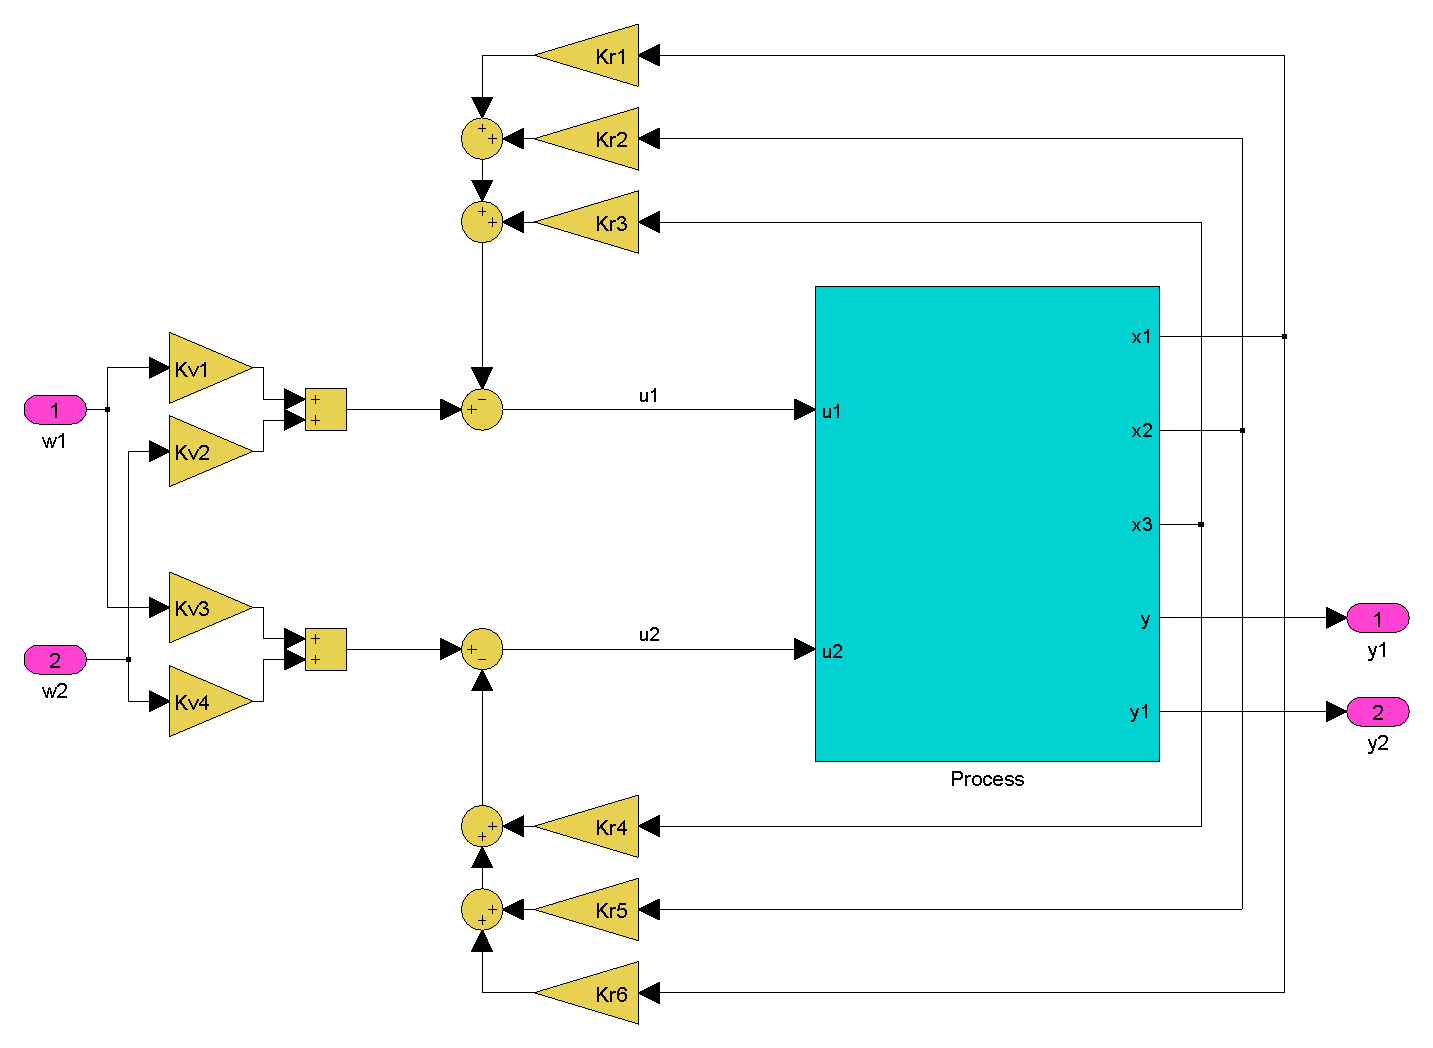
\includegraphics[width=1.00\textwidth]{03_Grafiken/MIMOprocess_controller.pdf}
	\caption{Principle model of a third order MIMO process including a state space controller}
	\label{fig:MIMOprocess_controller}
\end{figure}

Now in figure \ref{fig:MIMOprocess_controller} there is a simple MIMO-System. What exactly happens in the 'process-block' is not important, but there are two inputs \textit{u1} and \textit{u2}. Also, there are five outputs - three measured state variables \textit{x1}, \textit{x2} and \textit{x3} and the two outputs \textit{y1} and \textit{y2}. The state space controller, marked in yellowish brown, is a bit more complex than a state space controller for a SISO-System. So - how to calculate the state variable feedback factors and the pre-intensification factors now? Interesting answer, it is the same for MIMO-System as for SISO-Systems. The only thing is - it is more complex, because of more matrix equations, but those matrix equations are not the problem - therefore MATLAB is the tool.